\chapter{ANALISIS DAN PERANCANGAN}

\section{Model Desain}
    Secara garis besar, topik ini akan dibagi menjadi dua buah subsistem yang lebih kecil yakni \textit{resource allocator} dan DDS.
    Penjelasan lebih lanjut mengenai rincian desain subsistem dan pembagian kerja akan dibahas pada tabel \ref{tab:subsistemDivision}.
    \begin{table}[tbh]
        \caption{Pembagian Subsistem}\label{tab:subsistemDivision}
        \begin{center}
            \begin{tabular}{|m{0.5cm}|m{3cm}|m{5.5cm}|m{3cm}|}
                \hline
                \thead{No} & \thead{Subsistem} & \thead{Rincian Desain Subsistem} & \thead{Pembagian Kerja}\\
                \hline 
                1 & \textit{Resource Allocator} & \textit{Resource Allocator} berperan untuk melakukan alokasi \textit{bandwidth} secara tepat dan efisien yang bertujuan untuk meningkatkan rata-rata akurasi dari sistem \gls{vap} & Faishal Zharfan \\
                \hline 
                2 & DDS & DDS berperan dalam optimasi pengaturan konfigurasi parameter pengkodean dan kompresi video untuk mencapai akurasi inferensi terbaik. & Farhan Krishna\\
                \hline 
            \end{tabular}
        \end{center}
    \end{table}
    \subsection{\textit{Resource Allocator}}

    \begin{figure}[tbh]
        \centering
        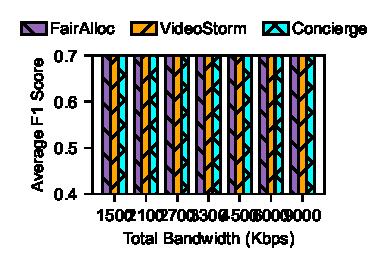
\includegraphics{./resources/concierge-perf.pdf}
        \caption{Tingkah Laku Sistem}\label{fig:resource_alloc_tes}
    \end{figure}
% \begin{algorithm}
%     \caption{An algorithm with caption}\label{alg:cap}
%     \begin{algorithmic}
%     \Require $n \geq 0$
%     \Ensure $y = x^n$
%     \State $y \gets 1$
%     \State $X \gets x$
%     \State $N \gets n$
%     \While{$N \neq 0$}
%     \If{$N$ is even}
%         \State $X \gets X \times X$
%         \State $N \gets \frac{N}{2}$  \Comment{This is a comment}
%     \ElsIf{$N$ is odd}
%         \State $y \gets y \times X$
%         \State $N \gets N - 1$
%     \EndIf
%     \EndWhile
%     \end{algorithmic}
%     \end{algorithm}

\section{Implementasi}
